
\documentclass[12pt,a4paper]{report}

%===========================================================
% PACKAGES
%===========================================================

\usepackage{graphicx}
\usepackage{float}
\usepackage{amsmath}
\usepackage{amssymb}
\usepackage{booktabs}
\usepackage{multirow}
\usepackage{array}
\usepackage{longtable}
\usepackage{tabularx}
\usepackage{caption}
\usepackage{subcaption}
\usepackage{enumitem}
\usepackage{hyperref}
\usepackage{geometry}
\usepackage{setspace}
\usepackage{fancyhdr}
\usepackage{tikz}
\usepackage{xcolor}
\usepackage{comment}

\usetikzlibrary{
	positioning,
	arrows.meta,
	calc,
	shapes.geometric,
	shapes.misc,
	fit,
	backgrounds,
	decorations.pathmorphing
}

\geometry{
	left=1in,
	right=1in,
	top=1in,
	bottom=1in
}

\setlength{\headheight}{15pt}
\onehalfspacing

%===========================================================
% HEADER
%===========================================================

\pagestyle{fancy}
\fancyhf{}
\fancyhead[L]{Internship Training Report}
\fancyhead[R]{NITK Surathkal}
\fancyfoot[C]{\thepage}

%===========================================================
% DOCUMENT
%===========================================================

\begin{document}
	
	%===========================================================
	% TITLE PAGE
	%===========================================================
	
	\begin{titlepage}
		
		\begin{center}
			
			\vspace*{1cm}
			
			{\Large \textbf{PRACTICAL TRAINING REPORT}}
			
			\vspace{1.2cm}
			
			{\Large
				\textbf{
					CARS-SF: A Context-Aware Autonomous Rural Service Slicing Framework
					for Private 5G Networks
				}
			}
			
			\vspace{2cm}
			
			Submitted in partial fulfillment of the requirements\\
			for the Summer Internship
			
			\vspace{1.5cm}
			
			\textbf{Submitted By}
			
			\vspace{0.4cm}
			
			\textbf{Bammidi Ketan Rao}
			
			Roll No.: 252CS006
			
			Department of Computer Science and Engineering
			
			\vspace{1.5cm}
			
			\vfill
			
			Department of Computer Science and Engineering
			
			National Institute of Technology Karnataka
			
			Surathkal -- 575025
			
			\vspace{0.6cm}
			
			Academic Year 2026--2027
			
		\end{center}
		
	\end{titlepage}
	
	
	%===========================================================
	% ABSTRACT
	%===========================================================
	
	\chapter*{Abstract}
	
Rural and remote communities depend on communication networks for
healthcare, education, agriculture, emergency response, and other
essential services. These services have different network requirements
and may need different priorities as the operating situation changes.
Conventional network slicing can provide different resource allocations,
but fixed policies cannot easily respond when these priorities change.

This work presents CARS-SF, a Context-Aware Autonomous Rural Service
Slicing Framework for private 5G networks. The proposed framework aims to
identify incoming traffic using SliceNet, combine the identified service
with the current operating context and network condition, and use this
information to make adaptive resource-allocation decisions through
reinforcement learning. Network monitoring provides feedback so that
future decisions can respond to changing conditions.

The internship focused on establishing the foundation for this
framework. A configurable Mininet-based rural network environment was
developed along with service-aware operational scenarios and a hybrid
traffic-generation pipeline. The Rural Service-aware Network Slice
Dataset (RSNSD) was created by combining network-flow characteristics
with service and scenario information, and an initial SliceNet
classification framework was established using this dataset. These
components provide the simulation, data, and traffic-classification
foundation for the subsequent development of adaptive resource
management and autonomous network control.

\vspace{0.4cm}

\noindent\textbf{Keywords:}
Private 5G, Rural Networks, Network Slicing, Service-aware Networking,
Context-aware Networking, Reinforcement Learning, SliceNet, RSNSD,
Autonomous Networks.
	
	
	%===========================================================
	% CONTENTS
	%===========================================================
	
	\clearpage
	\pagenumbering{roman}
	
	\tableofcontents
	
	\clearpage
	
	\listoffigures
	
	\clearpage
	
	\listoftables
	
	\clearpage
	
	\pagenumbering{arabic}
	\setcounter{page}{1}
	
	\chapter{Introduction}
	
	Today, many applications depend on a stable Internet connection, but all applications do not have the same requirements. This becomes more important in rural areas, where a common network may support online education, healthcare, agriculture, general Internet access and emergency communication. During normal conditions, these services can share the available resources, but during an emergency, critical services such as healthcare and emergency communication should receive higher priority. 
	
	Traditional networks mainly use fixed QoS rules and predefined resource allocation, which does not adapt well when traffic patterns or operating conditions changes. 5G network slicing and Software Defined Networking (SDN) provide mechanisms to separate and control resources for different services, but their decisions are still largely based on predefined policies. Machine Learning can identify the type of incoming traffic, but traffic classification alone cannot determine how important that traffic is under the current situation. For example, healthcare traffic may require higher priority during an emergency, while educational traffic may become more important during an examination or learning session. Hence, the network needs to understand both the traffic and the context in which it is operating.
	
	From the study of existing approaches, we identified that traffic classification, network slicing and intelligent resource allocation are often handled as separate problems, with limited integration between them. This led to the research gap for a framework that can combine these capabilities into a single closed-loop system. Therefore, this work proposes an AI-driven, context-aware 5G network framework in which incoming traffic is classified using SliceNet, contextual information is used to determine service priority, and a Reinforcement Learning (RL) agent dynamically adapts network resources according to the changing network conditions. The proposed approach aims to move from fixed resource allocation towards an adaptive network that can identify which services are important in the current scenario and provide them with better connectivity when required.

	
	
	
	
	%===========================================================
	% CHAPTER 1
	%===========================================================
	
	\chapter{Problem Motivation}
	\label{chap:introduction}
	

\section{Rural Mission-Critical Communication Scenario}
\label{sec:rural_scenario}

Rural areas depend on communication networks for many important services,
including healthcare, education, agriculture, emergency services, and
general Internet access. These services share the same network, but they
do not have the same needs. For example, healthcare and emergency
communication may need low delay and reliable delivery, education may
need more bandwidth during school hours, while general Internet traffic
can usually work with lower priority.


\begin{table}[H]
	\centering
	\caption{Representative rural services and their changing network
		requirements}
	\label{tab:service_requirements}
	\begin{tabular}{p{2.8cm} p{3.2cm} p{3.4cm} p{3.6cm}}
		\toprule
		\textbf{Service} &
		\textbf{Typical Requirement} &
		\textbf{Context Affecting Priority} &
		\textbf{Expected Network Behaviour} \\
		\midrule
		
		Healthcare &
		Low delay, reliability &
		Normal / Emergency / Disaster &
		Higher priority during critical events \\
		
		Education &
		Sustained bandwidth &
		School Hours &
		More resources during peak activity \\
		
		Agriculture &
		Periodic sensing and IoT traffic &
		Harvest Season &
		Support increased monitoring demand \\
		
		Emergency &
		Low delay, high reliability &
		Emergency / Disaster &
		Highest priority during critical conditions \\
		
		General Internet &
		Best-effort access &
		All scenarios &
		Use remaining available resources \\
		
		\bottomrule
	\end{tabular}
\end{table}

The needs of these services can also change with the situation. During
normal operation, network resources can be shared among different
services. During an emergency or disaster, however, healthcare and
emergency communication may become more important, while general
Internet traffic may have to use fewer resources. Similarly, education
or agriculture may need more resources during periods of high activity.
The main challenge is therefore that service priority cannot always be
fixed in advance; it must change according to the service, the current
situation, and the condition of the network.


This creates the need for a network that can understand what type of
traffic it is carrying, recognize the current situation, and adjust its
resource allocation accordingly. Private 5G provides a suitable
environment for this because its network resources and service policies
can be configured according to application needs.
	

%-----------------------------------------------------------
\section{Operational Challenge}
\label{sec:operational_challenge}
%-----------------------------------------------------------

Rural networks may have limited resources while the type and amount of
traffic can change with time and operating conditions. Network slicing
allows different services to share the same infrastructure with
different resource allocations \cite{kazmi2019slicing},
but fixed slice policies cannot automatically respond when service
priorities change. For example, during an emergency, healthcare and
emergency communication may require more resources, while general
Internet traffic may need to operate with lower priority.

	
\begin{figure}[H]
	\centering
	\resizebox{\linewidth}{!}{%
		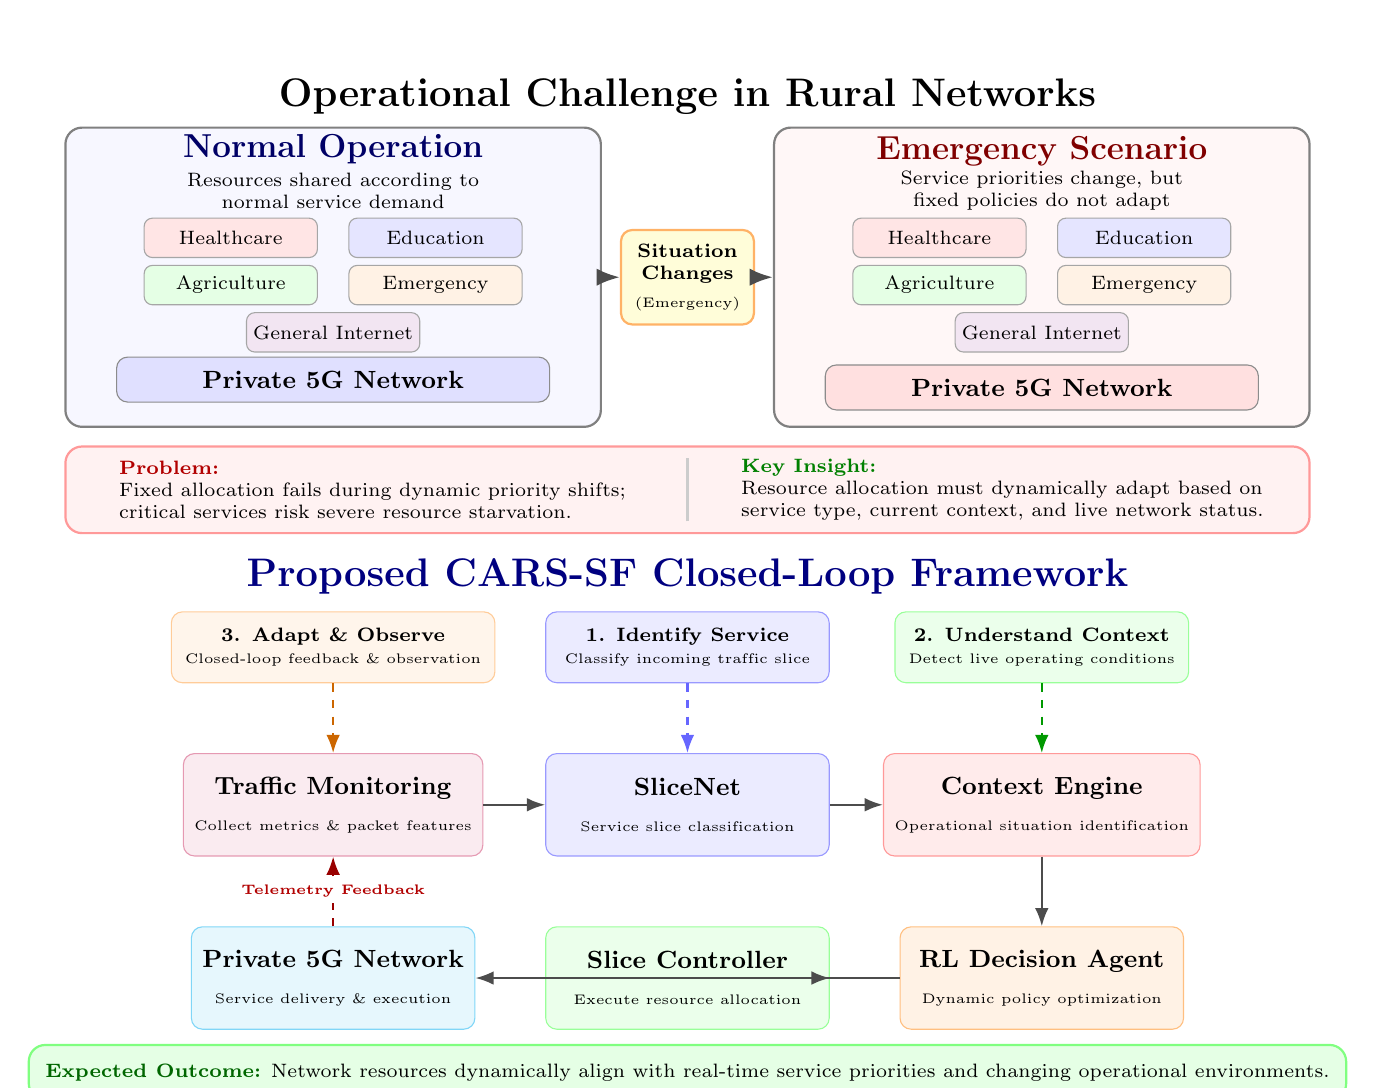
\begin{tikzpicture}[
			x=1cm,
			y=1cm,
			font=\small,
			>=Latex,
			panel/.style={
				rounded corners=6pt,
				draw=black!50,
				line width=0.8pt,
				inner sep=6pt
			},
			box/.style={
				rectangle,
				rounded corners=4pt,
				draw=black!45,
				align=center,
				inner sep=5pt
			},
			service/.style={
				rectangle,
				rounded corners=3pt,
				draw=black!35,
				minimum width=2.2cm,
				minimum height=0.5cm,
				align=center,
				font=\scriptsize,
				inner sep=2pt
			},
			module/.style={
				rectangle,
				rounded corners=4pt,
				draw=black!50,
				minimum width=2.4cm,
				minimum height=1.5cm,
				align=center,
				inner sep=4pt
			},
			arrow/.style={
				->,
				thick,
				black!70
			},
			dashedarrow/.style={
				->,
				thick,
				dashed,
				black!60
			}
			]
			
			% ========================================================
			% MAIN TITLE
			% ========================================================
			\node[font=\bfseries\Large, align=center] at (8, 0) {Operational Challenge in Rural Networks};
			
			% ========================================================
			% TOP SECTION: NORMAL vs EMERGENCY
			% ========================================================
			
			% Normal Operation Panel
			\node[panel, fill=blue!3, minimum width=6.8cm, minimum height=3.8cm] (normalpanel) at (3.5, -2.3) {};
			\node[font=\bfseries\large, color=blue!40!black] at (3.5, -0.68) {Normal Operation};
			\node[align=center, font=\scriptsize] at (3.5, -1.2) {Resources shared according to\\normal service demand};
			
			\node[service, fill=red!10] at (2.2, -1.8) {Healthcare};
			\node[service, fill=blue!10] at (4.8, -1.8) {Education};
			\node[service, fill=green!10] at (2.2, -2.4) {Agriculture};
			\node[service, fill=orange!10] at (4.8, -2.4) {Emergency};
			\node[service, fill=violet!10] at (3.5, -3.0) {General Internet};
			\node[box, fill=blue!12, minimum width=5.5cm] at (3.5, -3.6) {\textbf{Private 5G Network}};
			
			% Situation Transition
			\node[box, fill=yellow!15, draw=orange!60, line width=0.8pt, font=\bfseries\scriptsize, align=center] (change) at (8, -2.3) {Situation\\Changes\\[2pt]\normalfont\tiny (Emergency)};
			\draw[arrow, line width=1.2pt] (normalpanel.east) -- (change.west);
			
			% Emergency Scenario Panel
			\node[panel, fill=red!3, minimum width=6.8cm, minimum height=3.8cm] (emergpanel) at (12.5, -2.3) {};
			\node[font=\bfseries\large, color=red!50!black] at (12.5, -0.7) {Emergency Scenario};
			\node[align=center, font=\scriptsize] at (12.5, -1.2) {Service priorities change, but\\fixed policies do not adapt};
			
			\node[service, fill=red!10] at (11.2, -1.8) {Healthcare};
			\node[service, fill=blue!10] at (13.8, -1.8) {Education};
			\node[service, fill=green!10] at (11.2, -2.4) {Agriculture};
			\node[service, fill=orange!10] at (13.8, -2.4) {Emergency};
			\node[service, fill=violet!10] at (12.5, -3.0) {General Internet};
			\node[box, fill=red!12, minimum width=5.5cm] at (12.5, -3.7) {\textbf{Private 5G Network}};
			\draw[arrow, line width=1.2pt] (change.east) -- (emergpanel.west);
			
			% ========================================================
			% MIDDLE SECTION: PROBLEM & KEY INSIGHT
			% ========================================================
			\node[panel, fill=red!5, draw=red!40, minimum width=15.8cm, minimum height=1.1cm] (problem) at (8, -5.0) {};
			
			\node[align=left, font=\scriptsize] at (4.0, -5.0) {
				\textbf{\color{red!70!black}Problem:}\\
				Fixed allocation fails during dynamic priority shifts;\\
				critical services risk severe resource starvation.
			};
			
			\draw[line width=0.8pt, black!20] (8, -5.4) -- (8, -4.6);
			
			\node[align=left, font=\scriptsize] at (12.0, -5.0) {
				\textbf{\color{green!50!black}Key Insight:}\\
				Resource allocation must dynamically adapt based on\\
				service type, current context, and live network status.
			};
			
			% ========================================================
			% BOTTOM SECTION: PROPOSED SOLUTION (3x3 GRID ORIENTATION)
			% ========================================================
			\node[font=\bfseries\Large, color=blue!50!black] at (8.0, -6.1) {Proposed CARS-SF Closed-Loop Framework};
			
			% --------------------------------------------------------
			% ROW 1: System Requirements (Inputs)
			% --------------------------------------------------------
			\node[box, fill=orange!8, draw=orange!40, minimum width=3.6cm, minimum height=0.9cm, align=center, font=\scriptsize] (req3) at (3.5, -7.0) {
				\textbf{3. Adapt \& Observe}\\
				\tiny Closed-loop feedback \& observation
			};
			
			\node[box, fill=blue!8, draw=blue!40, minimum width=3.6cm, minimum height=0.9cm, align=center, font=\scriptsize] (req1) at (8.0, -7.0) {
				\textbf{1. Identify Service}\\
				\tiny Classify incoming traffic slice
			};
			
			\node[box, fill=green!8, draw=green!40, minimum width=3.6cm, minimum height=0.9cm, align=center, font=\scriptsize] (req2) at (12.5, -7.0) {
				\textbf{2. Understand Context}\\
				\tiny Detect live operating conditions
			};
			
			% --------------------------------------------------------
			% ROW 2: Perception & Classification (Left -> Right)
			% --------------------------------------------------------
			\node[module, fill=purple!8, draw=purple!40, minimum width=3.6cm, minimum height=1.3cm] (monitor) at (3.5, -9.0) {
				\textbf{Traffic Monitoring}\\[2pt]
				\tiny Collect metrics \& packet features
			};
			
			\node[module, fill=blue!8, draw=blue!40, minimum width=3.6cm, minimum height=1.3cm] (slicenet) at (8.0, -9.0) {
				\textbf{SliceNet}\\[2pt]
				\tiny Service slice classification
			};
			
			\node[module, fill=red!8, draw=red!40, minimum width=3.6cm, minimum height=1.3cm] (context) at (12.5, -9.0) {
				\textbf{Context Engine}\\[2pt]
				\tiny Operational situation identification
			};
			
			% --------------------------------------------------------
			% ROW 3: Decision, Control & Execution (Right -> Left)
			% --------------------------------------------------------
			\node[module, fill=cyan!10, draw=cyan!50, minimum width=3.6cm, minimum height=1.3cm] (network) at (3.5, -11.2) {
				\textbf{Private 5G Network}\\[2pt]
				\tiny Service delivery \& execution
			};
			
			\node[module, fill=green!8, draw=green!40, minimum width=3.6cm, minimum height=1.3cm] (controller) at (8.0, -11.2) {
				\textbf{Slice Controller}\\[2pt]
				\tiny Execute resource allocation
			};
			
			\node[module, fill=orange!10, draw=orange!50, minimum width=3.6cm, minimum height=1.3cm] (rl) at (12.5, -11.2) {
				\textbf{RL Decision Agent}\\[2pt]
				\tiny Dynamic policy optimization
			};
			
			% --------------------------------------------------------
			% Connections & Serpentine Closed-Loop Flow
			% --------------------------------------------------------
			% Vertical Requirement Injections (Row 1 -> Row 2)
			\draw[dashedarrow, color=orange!80!black] (req3.south) -- (monitor.north);
			\draw[dashedarrow, color=blue!60] (req1.south) -- (slicenet.north);
			\draw[dashedarrow, color=green!60!black] (req2.south) -- (context.north);
			
			% Row 2 Forward Flow (Left to Right)
			\draw[arrow] (monitor.east) -- (slicenet.west);
			\draw[arrow] (slicenet.east) -- (context.west);
			
			% Downward Transition (Col 3: Row 2 -> Row 3)
			\draw[arrow] (context.south) -- (rl.north);
			
			% Row 3 Action Flow (Right to Left)
			\draw[arrow] (rl.west) -- (controller.west |- rl.west) -- (controller.east);
			\draw[arrow] (controller.west) -- (network.east);
			
			% Upward Closed-Loop Feedback Path (Col 1: Row 3 -> Row 2)
			\draw[->, thick, dashed, red!60!black] (network.north) -- (monitor.south) 
			node[midway, fill=white, inner sep=2pt, font=\tiny\bfseries, text=red!70!black] {Telemetry Feedback};
			% Outcome Summary Box
			\node[panel, fill=green!10, draw=green!50, minimum width=15.8cm, minimum height=0.7cm, font=\scriptsize] at (8, -12.4) {
				\textbf{\color{green!40!black}Expected Outcome:} Network resources dynamically align with real-time service priorities and changing operational environments.
			};
			
		\end{tikzpicture}%
	}
	\caption{Operational challenge in rural networks and the proposed CARS-SF closed-loop framework for service-aware and context-aware resource management.}
	\label{fig:cars_sf_framework}
\end{figure}

Standard 5G service categories such as eMBB, URLLC, and mMTC provide
broad descriptions of communication needs, but do
not directly identify the application generating the traffic or its
importance in a specific situation. The network therefore needs to
understand both the service being carried and the current operating
condition before deciding how resources should be distributed.
Research on intelligent slicing and reinforcement learning has already
explored dynamic resource allocation under changing network conditions.



%-----------------------------------------------------------
\section{Research Problem and Identified Research Gap}
\label{sec:research_gap}
%-----------------------------------------------------------

This creates three basic requirements for CARS-SF: the network must
identify the service generating the traffic, understand the current
situation, and adjust its resources accordingly. It must also monitor
the result so that future decisions can respond to changes in the
network \cite{moysen2018selforganized}. Therefore, the main problem is
how to make network resource allocation change according to the service,
the current situation, and the network condition.

Based on this, the research problem addressed in this work is:

\begin{quote}
	\emph{How can a private 5G network serving different rural services
		identify the service generating the traffic, understand the current
		situation, and adjust network resources according to the changing
		needs of those services?}
\end{quote}

Existing research has already addressed important parts of this
problem. Network slicing allows different services to share the same
infrastructure with different resource and QoS requirements
\cite{kazmi2019slicing}. Machine-learning-based traffic
classification can identify the type of service from network traffic. Reinforcement learning has
also been studied for changing resource allocation and network-slice
management \cite{li2018drl,yan2019irs,sciancalepore2019rlnsb}. These
works show that the individual components required for an adaptive
network are possible. However, they do not by themselves provide the
complete service--context--decision--feedback loop required for the
rural scenario considered in this work.

The gap identified from this study is therefore mainly an
\textbf{integration gap}. The network needs to know \emph{what service
	is being carried}, \emph{what is happening in the current situation},
and \emph{what the network condition is} before deciding how resources
should be allocated. After the action is applied, the network must also
observe its effect and use that information for the next decision.
Recent work has demonstrated real-time service-aware slice adaptation
using traffic classification and network information
\cite{tsourdinis2024serviceaware}, but the CARS-SF problem further
considers changing service priority based on the operational situation
of the rural network.

\begin{table}[H]
	\centering
	\caption{Literature-derived capabilities and resulting CARS-SF
		design requirements}
	\label{tab:literature_gap}
	\begin{tabular}{p{3.0cm} p{4.3cm} p{4.3cm}}
		\toprule
		\textbf{Capability} &
		\textbf{Existing Contribution} &
		\textbf{Requirement for CARS-SF} \\
		\midrule
		
		Network Slicing &
		Logical isolation and different QoS over shared infrastructure
		\cite{kazmi2019slicing} &
		Dynamic service-level resource allocation \\
		
		Service-aware Slicing &
		Considers application requirements during slice management
		 &
		Service information in resource decisions \\
		
		Traffic Classification &
		Identifies service or application characteristics from network flows
		\cite{xie2021traffic,mohammedali2022traffic} &
		Service perception through SliceNet \\
		
		RL-based Management &
		Adapts resource allocation under changing network conditions
		\cite{li2018drl,sciancalepore2019rlnsb} &
		Context-aware adaptive decisions \\
		
		Autonomous Networking &
		Uses monitoring and feedback for network adaptation
		\cite{moysen2018selforganized} &
		Continuous closed-loop operation \\
		
		\bottomrule
	\end{tabular}
\end{table}



CARS-SF is therefore designed to connect these capabilities within one
framework. SliceNet provides information about the service represented
by incoming traffic, the context layer represents the current operating
situation, and the reinforcement learning component provides the
adaptive resource-management decision. Network monitoring provides the
feedback required to evaluate each decision. The framework consequently
moves from simply assigning traffic to predefined slices towards
resource allocation that can respond to the service, situation, and
condition of the network.
%-----------------------------------------------------------
\section{Research Objective}
\label{sec:research_objective}
%-----------------------------------------------------------

The objective of CARS-SF is to develop a framework that can manage
network resources according to the service being carried and the current
operating situation in a rural private 5G network. The framework aims to
identify incoming traffic, understand its importance in the current
situation, adjust network resources accordingly, and monitor the result.
This creates a continuous cycle in which network decisions can change as
the traffic and operating conditions change.

The internship focuses on establishing the foundation for this framework.
This includes developing a configurable Mininet-based rural network
environment, modelling different services and operating scenarios,
creating the Rural Service-aware Network Slice Dataset (RSNSD), and
developing the initial SliceNet traffic-classification framework.
	
\chapter{Background and Literature Study}
\label{chap:background}
%-----------------------------------------------------------
%-----------------------------------------------------------
\section{Private 5G for Rural and Mission-Critical Applications}
\label{sec:private5g}
%-----------------------------------------------------------

Private 5G networks provide greater control over network resources,
Quality of Service (QoS), security, and service management than
conventional public networks.
This makes them suitable for environments where different services
share the same network but have different communication requirements.

This is particularly relevant in rural areas, where a common network
may support healthcare, education, agriculture, public services, and
emergency communication. Previous work has also studied network
slicing as a way to support multiple rural services over shared 5G
infrastructure, while 5G-based communication
has been explored for applications such as agriculture.

For CARS-SF, private 5G therefore provides the network environment in
which service-specific policies and resource allocation can be
controlled and adapted. It forms the underlying platform for the
service-aware and context-aware resource management proposed in this
work.
	
%-----------------------------------------------------------
\section{Network Slicing and Service Differentiation}
\label{sec:network_slicing}
%-----------------------------------------------------------

Network slicing allows different services to share the same 5G
infrastructure while receiving different resource and Quality of Service
(QoS) requirements \cite{kazmi2019slicing}. Standard
categories such as eMBB, URLLC, and mMTC provide broad service
classifications, but rural networks may need to distinguish between
specific applications such as healthcare, education, agriculture, and
emergency communication. Service-aware slicing therefore considers the
requirements of individual services when managing network resources

For CARS-SF, this means that the network must first know which service
is generating the traffic before deciding how its resources should be
managed. This creates the need for a traffic-classification layer that
can identify services from observed network traffic.

\begin{table}[H]
	\centering
	\caption{Selected literature on intelligent traffic classification
		and adaptive network resource management}
	\label{tab:intelligent_network_management}
	\begin{tabular}{p{2.5cm} p{3.4cm} p{4.1cm} p{3.2cm}}
		\toprule
		\textbf{Work} &
		\textbf{Area} &
		\textbf{Main Contribution} &
		\textbf{Relevance to CARS-SF} \\
		\midrule
		
		Xie \textit{et al.} \cite{xie2021traffic} &
		Traffic Classification &
		Uses machine learning to classify traffic associated with 5G
		network slices. &
		Supports service-aware traffic perception. \\
		
		Mohammedali \textit{et al.} \cite{mohammedali2022traffic} &
		Traffic Classification &
		Applies deep learning for traffic classification in
		end-to-end 5G/B5G slice management. &
		Connects traffic classification with slice management. \\
		
		Li \textit{et al.} \cite{li2018drl} &
		Reinforcement Learning &
		Uses deep reinforcement learning for dynamic resource
		management in network slicing. &
		Provides the basis for adaptive resource decisions. \\
		
		Yan \textit{et al.} \cite{yan2019irs} &
		RAN Resource Management &
		Applies intelligent resource scheduling to 5G RAN slicing. &
		Supports dynamic resource allocation. \\
		
		Sciancalepore \textit{et al.} \cite{sciancalepore2019rlnsb} &
		Slice Management &
		Uses reinforcement learning for network-slice broker decisions. &
		Supports adaptive slice-level control. \\
		
		Moysen and Giupponi \cite{moysen2018selforganized} &
		Autonomous Networking &
		Studies machine learning for self-organized network management. &
		Supports the monitoring and adaptation concept. \\
		
		\bottomrule
	\end{tabular}
\end{table}


%-----------------------------------------------------------
\section{Intelligent Traffic Perception and Autonomous Resource Management}
\label{sec:intelligent_network_management}
%-----------------------------------------------------------

Machine-learning-based traffic classification can identify the service
represented by network traffic using observable flow characteristics
\cite{xie2021traffic,mohammedali2022traffic}. For CARS-SF, this forms the
perception stage, where SliceNet converts incoming network observations
into service information that can be used by the network-management
system.

Reinforcement learning provides a way to make resource-allocation
decisions based on the current network condition instead of relying
only on fixed rules. Previous studies have explored RL for dynamic
resource allocation and network-slice management under changing traffic
conditions \cite{li2018drl, sciancalepore2019rlnsb}. In
CARS-SF, the RL agent is intended to use service information, operating
context, and network conditions to decide how available resources
should be adjusted.

These two capabilities can be combined with continuous network
monitoring to form a closed loop. The network observes traffic,
identifies the service, makes a resource-allocation decision, applies
the change, and observes the resulting network behaviour. This follows
the broader idea of autonomous network management, where monitoring and
adaptation reduce dependence on fixed policies
\cite{moysen2018selforganized}. This closed-loop approach forms the
basis of the CARS-SF framework and its future extension towards
self-healing network operation.
	


	\chapter{Internship Engineering Work}
	\label{chap:internship_work}
	
	The internship focused on establishing the experimental and data
	foundation required for the CARS-SF framework. The work resulted in a
	reproducible rural network environment, representative service and
	operational scenarios, a service-aware network dataset, and the initial
	traffic-classification pipeline.
	\begin{comment}
	\begin{figure}
		\centering
		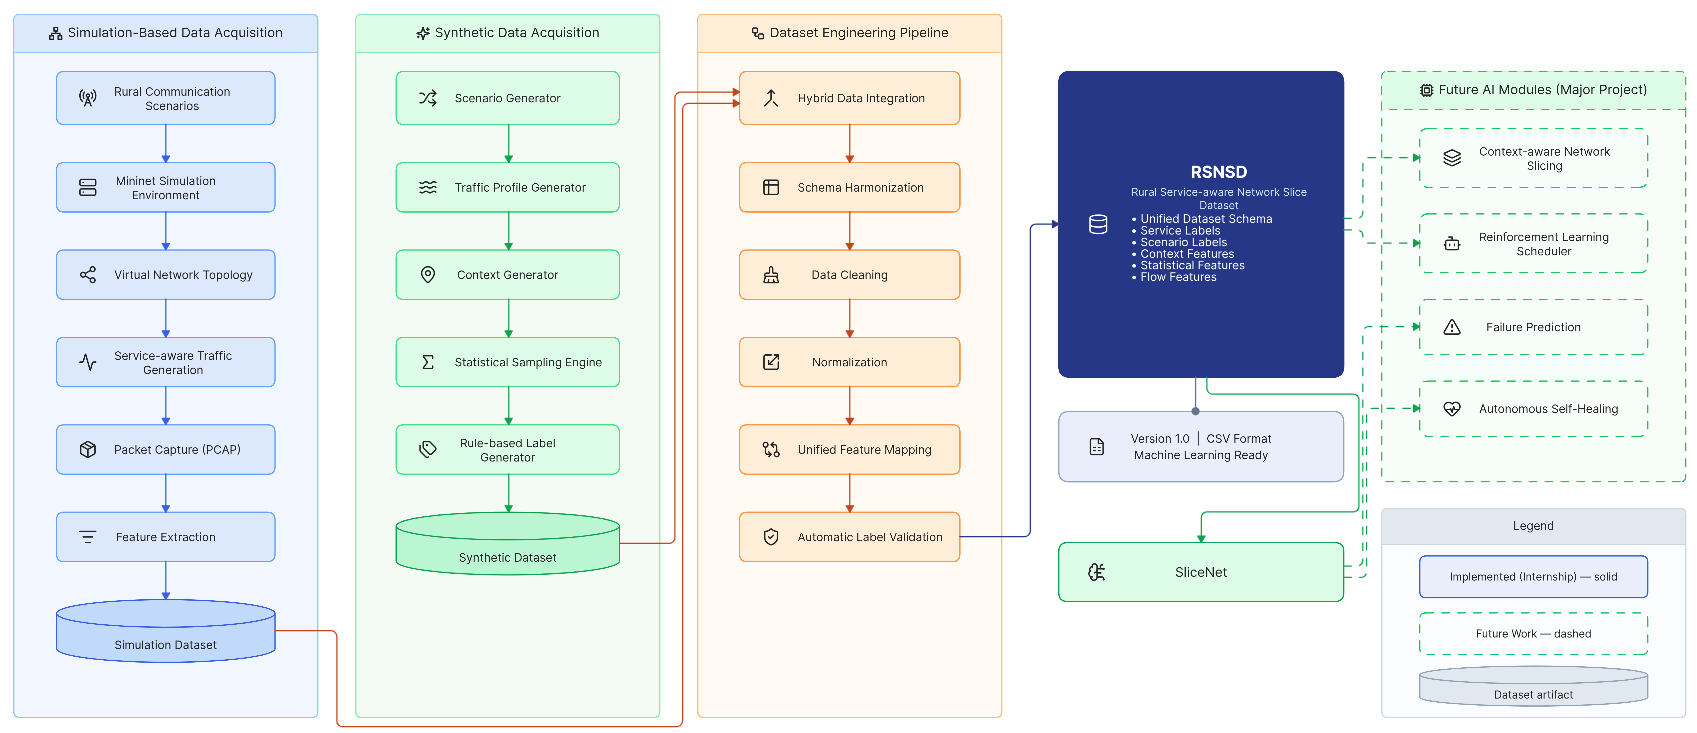
\includegraphics[width=0.5\linewidth]{screenshot004}
		\caption{}
		\label{fig:dataset}
	\end{figure}
\end{comment}
	%-----------------------------------------------------------
	\section{Experimental Environment and Scenario Modeling}
	\label{sec:experimental_environment}
	%-----------------------------------------------------------
	
	A configurable Mininet-based network environment was developed to
	emulate the communication characteristics of a rural deployment without
	requiring dedicated physical 5G hardware. The environment incorporates
	service-specific hosts, Open vSwitch-based forwarding, configurable
	network links, traffic generation, and network monitoring, providing a
	controlled platform for generating and observing heterogeneous service
	traffic.
	
		
	
	The environment was configured to represent different operational
	conditions in which service demand and relative priorities can change.
	The implemented scenarios include normal operation, increased
	education-related activity during school hours, elevated agricultural
	and IoT activity during the harvest season, emergency operation with
	greater priority for critical services, and disaster recovery under
	constrained resource availability. These scenarios provide the
	contextual variation required for evaluating service-aware network
	management.
	
	
	%-----------------------------------------------------------
	\section{RSNSD: Rural Service-aware Network Slice Dataset}
	\label{sec:rsnsd}
	%-----------------------------------------------------------
	
	To support service-aware traffic analysis, a hybrid traffic-generation
	and data-collection pipeline was established by combining
	simulation-derived network traffic with statistically generated
	synthetic traffic. The resulting Rural Service-aware Network Slice
	Dataset (RSNSD) captures network-flow characteristics together with
	service and operational context, providing a unified data foundation
	for the machine-learning components of CARS-SF.
	
	\begin{figure}
		\centering
		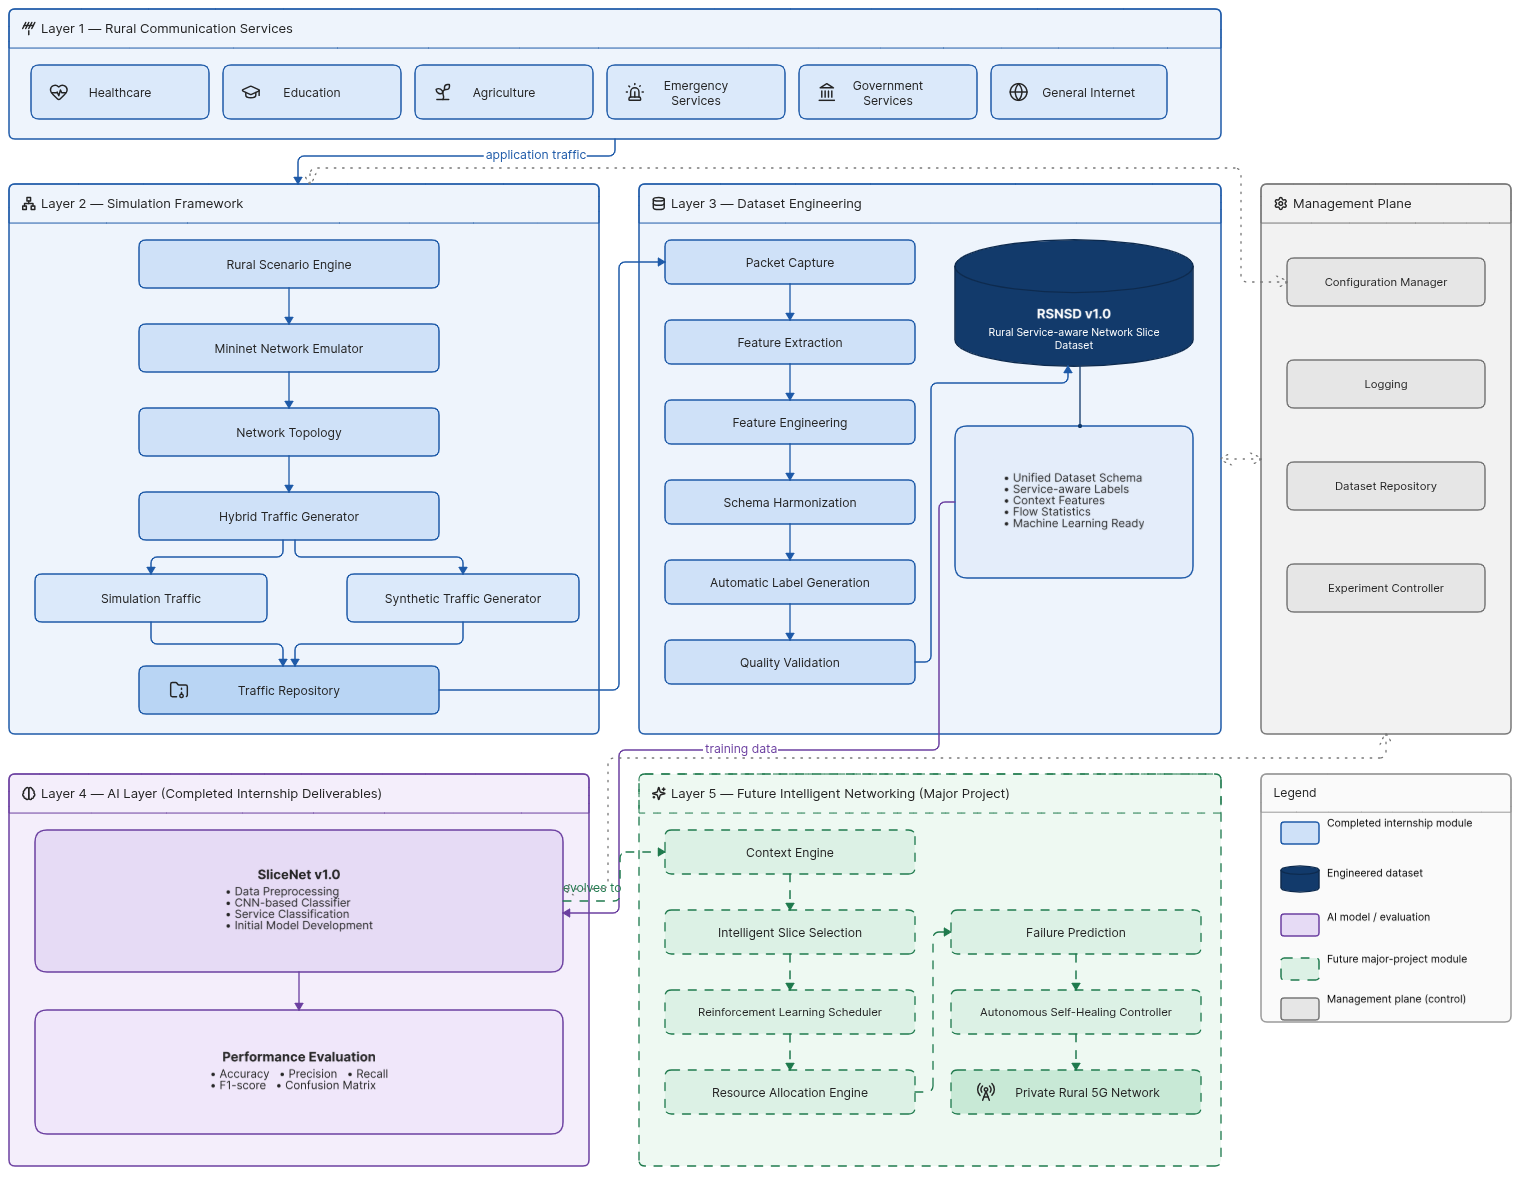
\includegraphics[width=1\linewidth]{screenshot005}
		\caption{Dataset engineering and data flow architecture}
		\label{fig:layered_approach}
	\end{figure}
	
	
	The dataset incorporates representative Layer 2--4 features, flow and
	temporal statistics, service labels, operational scenarios, and
	associated QoS priorities. This representation allows network
	observations to be related not only to their measurable traffic
	characteristics, but also to the service and context they represent.
	
	
	%-----------------------------------------------------------
	\section{SliceNet Engineering Foundation}
	\label{sec:slicenet_foundation}
	%-----------------------------------------------------------
	
	SliceNet was formulated as the service-perception component of
	CARS-SF, using RSNSD to frame traffic classification as a supervised
	multi-class learning problem. The internship established the
	classification pipeline, including feature representation,
	preprocessing, model formulation, and the interface required for
	integration with subsequent network-management components.
	
	The resulting environment, dataset, and SliceNet foundation establish
	the perception and experimentation layers of CARS-SF. The integration
	of this perception layer with context-aware resource orchestration and
	reinforcement learning-based network control forms the subsequent
	development direction of the major project.
	
	\begin{table}[H]
		\centering
		\caption{Internship deliverables and their role in the CARS-SF framework}
		\label{tab:internship_dod}
		\begin{tabular}{p{3.2cm} p{5.2cm} p{4.0cm}}
			\toprule
			\textbf{Deliverable} &
			\textbf{Engineering Work Established} &
			\textbf{Role in CARS-SF} \\
			\midrule
			
			Mininet Rural Environment &
			Configurable topology, service-specific hosts, OVS forwarding,
			traffic generation, and monitoring &
			Experimental foundation \\
			
			Operational Scenarios &
			Normal operation, school hours, harvest season, emergency, and
			disaster recovery &
			Context representation \\
			
			Traffic Generation Pipeline &
			Simulation-derived and synthetic service traffic &
			Representative network observations \\
			
			RSNSD &
			L2--L4, flow, temporal, service, context, and QoS information &
			Machine-learning data foundation \\
			
			SliceNet Foundation &
			Feature representation, preprocessing, and supervised
			service-classification pipeline &
			Service-perception layer \\
			
			\bottomrule
		\end{tabular}
	\end{table}
\chapter{Conclusion and Future Direction}
\label{chap:conclusion}

The internship established the main engineering components required for
the CARS-SF framework. A configurable Mininet-based rural network
environment was developed to represent different services and operating
conditions. It supports service-specific traffic generation,
configurable network settings, and network monitoring, providing the
environment needed for further experiments.

The Rural Service-aware Network Slice Dataset (RSNSD) was then developed
using simulation-based and synthetic traffic. The dataset links network
flow features with service classes, operating scenarios, and QoS
priorities, providing the data required for service-aware traffic
classification.

The initial SliceNet framework was also established using RSNSD to
classify incoming traffic into service categories. Thus, the internship
delivered three main outcomes: the rural network simulation environment,
the RSNSD dataset, and the initial SliceNet classification pipeline.
Together, these provide the simulation, data, and service-classification
base required for the next stage of CARS-SF.

The remaining major-project work will build on these components by
integrating them with the private 5G environment, context-aware resource
management, and reinforcement learning-based control. The final system
will be evaluated under changing service demands and operating
conditions, with dynamic resource adaptation and self-healing forming
the longer-term direction of the framework.
	
	
	%===========================================================
	% REFERENCES
	%===========================================================
%===========================================================
% REFERENCES
%===========================================================

\begin{thebibliography}{99}
\bibitem{kazmi2019slicing}
S. M. A. Kazmi, L. U. Khan, N. H. Tran, and C. S. Hong,
\textit{Network Slicing for 5G and Beyond Networks}.
Cham, Switzerland: Springer, 2019.

\bibitem{wangserviceaware}
R. Wang, A. H. Aghvami, and V. Friderikos,
``Service-aware design policy of end-to-end network slicing for 5G use
cases,'' 2018.

\bibitem{xie2021traffic}
F. Xie, D. Wei, and Z. Wang,
``Traffic analysis for 5G network slice based on machine learning,''
\textit{EURASIP Journal on Wireless Communications and Networking},
2021.

\bibitem{mohammedali2022traffic}
N. A. Mohammedali, T. Kanakis, A. Al-Sherbaz, and M. O. Agyeman,
``Traffic classification using deep learning approach for end-to-end
slice management in 5G/B5G,'' 2022.

\bibitem{li2018drl}
R. Li \textit{et al.},
``Deep reinforcement learning for resource management in network
slicing,'' \textit{IEEE Access}, vol. 6, pp. 74429--74441, 2018.

\bibitem{yan2019irs}
M. Yan, G. Feng, J. Zhou, Y. Sun, and Y.-C. Liang,
``Intelligent resource scheduling for 5G radio access network slicing,''
\textit{IEEE Transactions on Vehicular Technology}, vol. 68, no. 8,
pp. 7691--7703, 2019,
doi:10.1109/TVT.2019.2922668.

\bibitem{sciancalepore2019rlnsb}
V. Sciancalepore, X. Costa-Perez, and A. Banchs,
``RL-NSB: Reinforcement learning-based 5G network slice broker,''
\textit{IEEE/ACM Transactions on Networking}, vol. 27, no. 4,
pp. 1543--1557, 2019.

\bibitem{moysen2018selforganized}
J. Moysen and L. Giupponi,
``From 4G to 5G: Self-organized network management meets machine
learning,'' \textit{Computer Communications}, vol. 129,
pp. 248--268, 2018.
	
\end{thebibliography}
	
\end{document}
